\section{段落・数式・浮動体のレイアウトパラメータ}

\subsection{段落レイアウト}

\begin{figure}[htbp]
 \begin{center}
  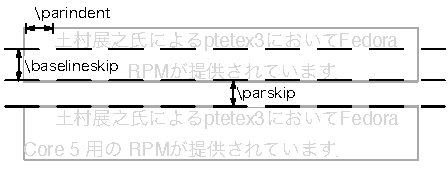
\includegraphics{layout-paragraph}
  \caption{段落設定のパラメータ}\figlab{段落設定のパラメータ}
 \end{center}
\end{figure}

\subsection{インデントを設定する}

\subsection{段落同士の空きを調整する}



\subsection{数式レイアウト}

\begin{figure}[htbp]
 \begin{center}
  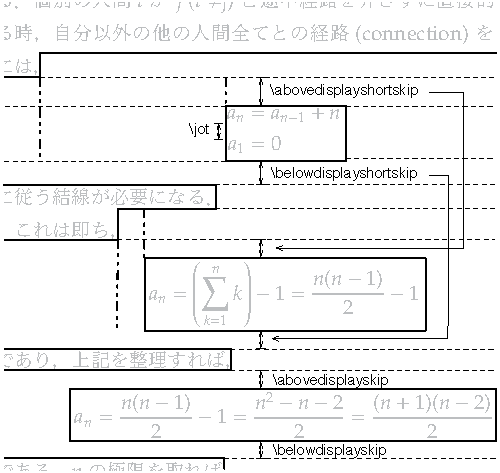
\includegraphics{layout-math}
  \caption{数式レイアウトのパラメータ}\figlab{数式レイアウトのパラメータ}
 \end{center}
\end{figure}

\subsection{fleqn}

\begin{figure}[htbp]
 \begin{center}
  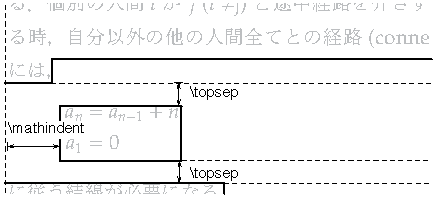
\includegraphics{layout-math-fleqn}
  \caption{fleqn数式レイアウトのパラメータ}\figlab{fleqn数式レイアウトのパラメータ}
 \end{center}
\end{figure}

\subsection{浮動体配置のパラメータ}

\begin{figure}[htbp]
 \begin{center}
  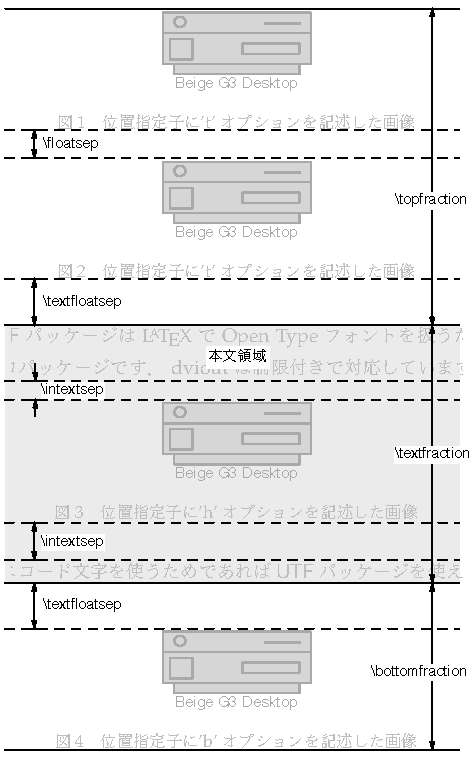
\includegraphics{layout-float}
  \caption{浮動体配置のパラメータ}\figlab{浮動体配置のパラメータ}
 \end{center}
\end{figure}


\C{dbltopnumber}
\C{dbltopfraction}
\C{dblfloatpagefraction}
\C{dblfloatsep}
\C{dbltextfloatsep}


\subsection{浮動体だけのページの書式パラメータ}

\C{floatpagefraction}
表が占めるべき最低の割合.